\chapter{Sample Performance Metrics}

In this section, we present the results of a pair of nodes with inter node distance at the median of all the node pairs in the simulation volume. There are 36 nodes randomly distributed the flying volume and the simulation state is the same as in Section \ref{pdr}.


In \fref{fig:med_fl_dr} we can notice that the PDR exceeds 90\% for HTL greater than two. This can also be confirmed in \fref{fig:med_pe_hops} where the average number of hops made by successfully delivered packets is approximately equal to two. Due to the small number of hops there is no noticeable difference for the packet delivery ratio in single or diverged transmission zones. Moreover, the average number of transmissions increase for flooding because increase in total number of transmissions is much higher than increase in delivery ratio.

\begin{figure}
\centering
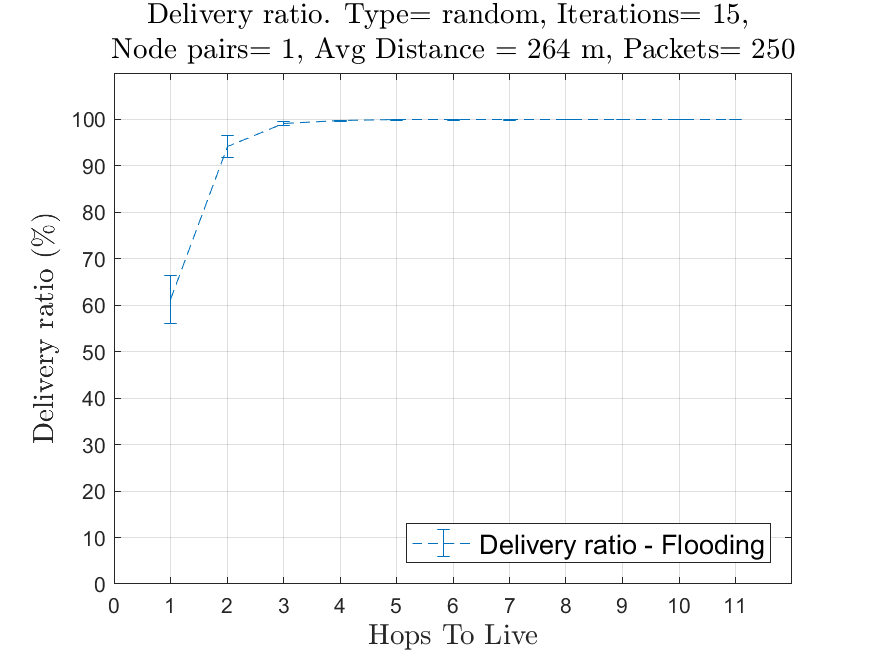
\includegraphics[width=1\textwidth]{ncsuthesis-0.6/Appendix-A/figs/median_fl_DR_random.png}
\caption{Packet delivery ratio in random node distribution for flooding algorithm for median inter drone separation}
\label{fig:med_fl_dr}
\end{figure}

\begin{figure}
\centering
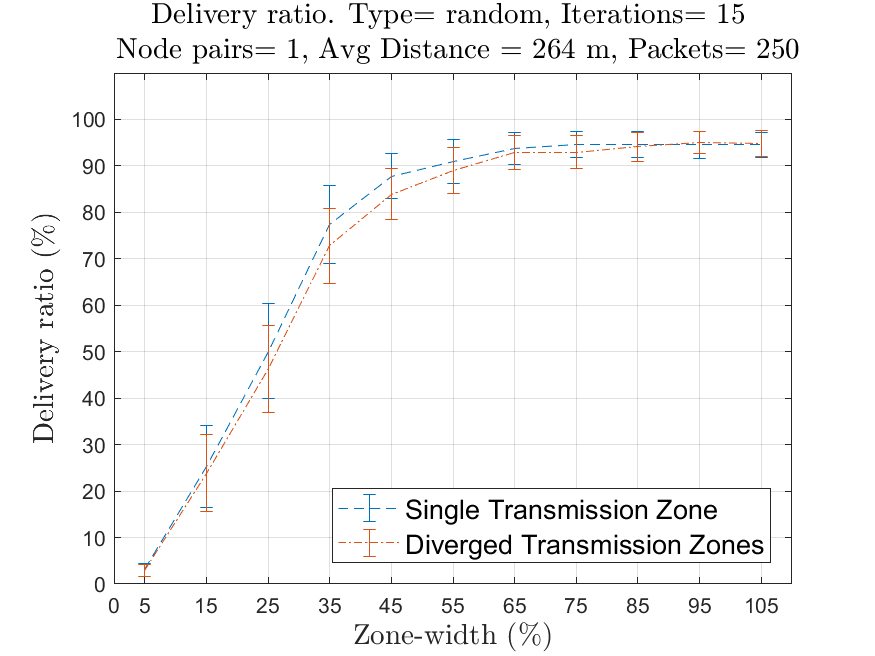
\includegraphics[width=1\textwidth]{ncsuthesis-0.6/Appendix-A/figs/median_pe_DR_random.png}
\caption{Packet delivery ratio in random node distribution for petal routing for median inter drone separation}
\label{fig:med_pe_dr}
\end{figure}

\begin{figure}
\centering
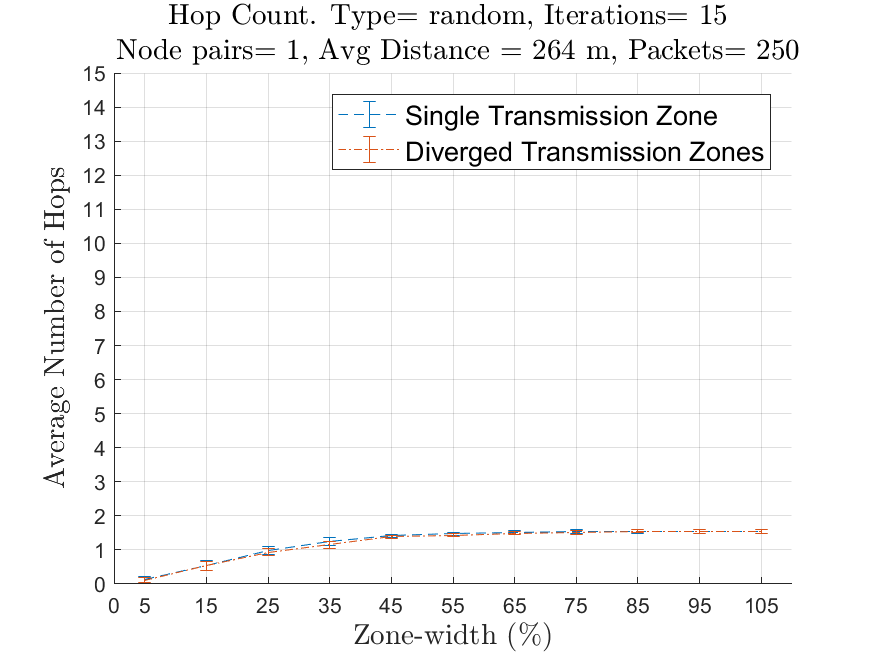
\includegraphics[width=1\textwidth]{ncsuthesis-0.6/Appendix-A/figs/median_pe_hops_random.png}
\caption{Average number of hops by successfully delivered packets}
\label{fig:med_pe_hops}
\end{figure}

\begin{figure}
\centering
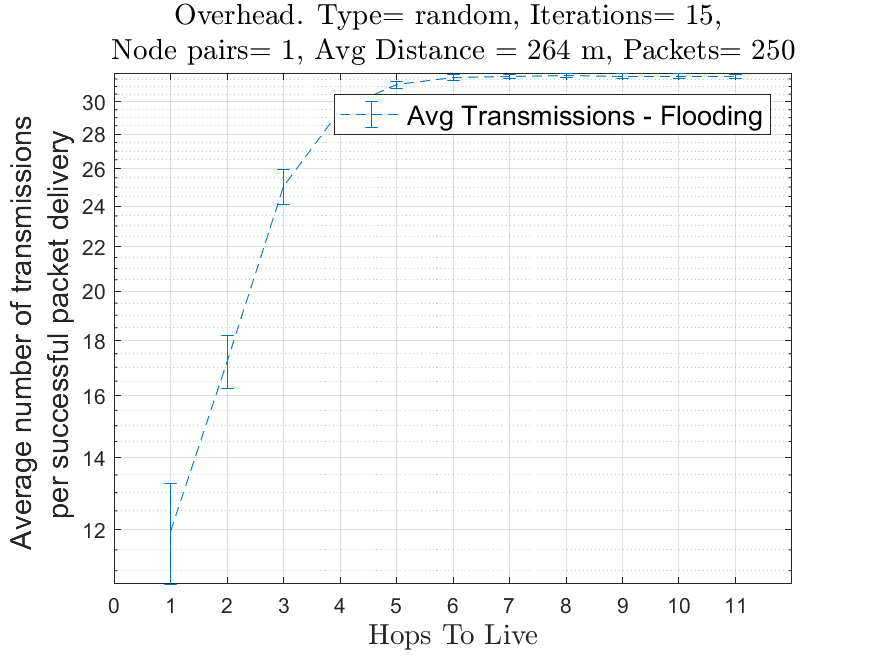
\includegraphics[width=1\textwidth]{ncsuthesis-0.6/Appendix-A/figs/median_fl_trans_random.png}
\caption{Average number of transmissions per successful packet delivery in random node distribution for flooding algorithm}
\label{fig:med_fl_trans}
\end{figure}

\begin{figure}
\centering
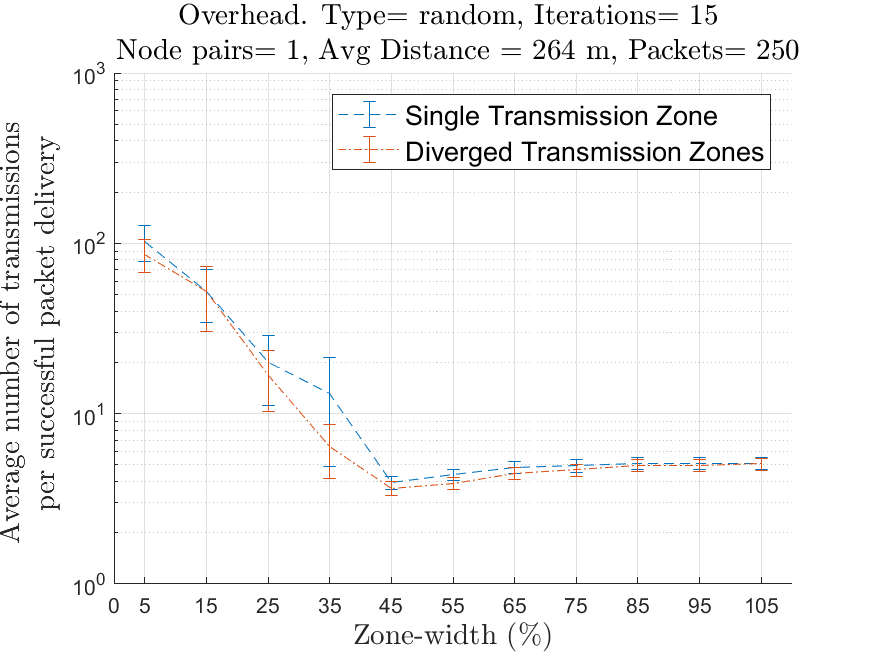
\includegraphics[width=1\textwidth]{ncsuthesis-0.6/Appendix-A/figs/medianpe_trans_random.png}
\caption{Average number of transmissions per successful packet delivery in random node distribution for petal routing}
\label{fig:med_pe_trans}
\end{figure}

